% Inactive historical alternative. Canonical source: Fig-2.svg (see README.md).
\documentclass[tikz,border=2pt]{standalone}
\usepackage[T1]{fontenc}
\usepackage{amsmath}
\usetikzlibrary{arrows.meta,positioning,fit}
\begin{document}
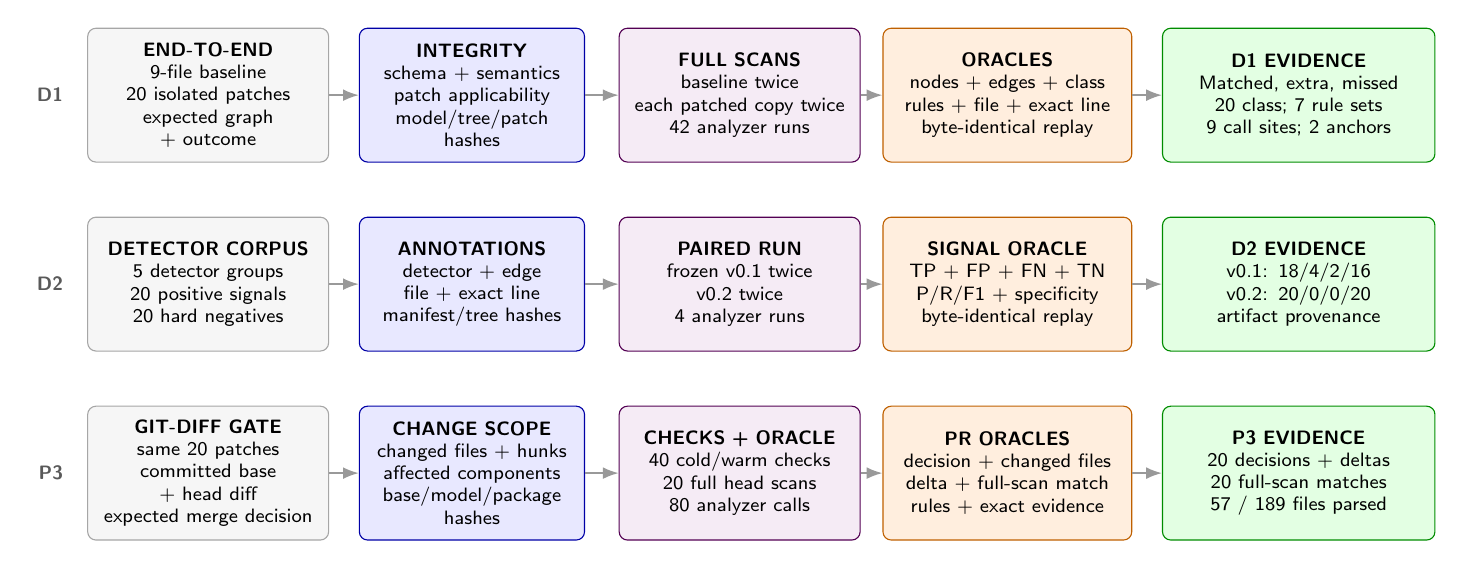
\begin{tikzpicture}[
    every node/.style={font=\sffamily\scriptsize},
    stage/.style={rounded corners=3pt, align=center, inner xsep=1.8mm, inner ysep=1.7mm, minimum height=17mm},
    data/.style={stage, draw=gray!70, fill=gray!7, text width=27mm},
    gate/.style={stage, draw=blue!65!black, fill=blue!9, text width=25mm},
    run/.style={stage, draw=violet!65!black, fill=violet!8, text width=27mm},
    verify/.style={stage, draw=orange!75!black, fill=orange!13, text width=28mm},
    output/.style={stage, draw=green!55!black, fill=green!11, text width=31mm},
    row label/.style={font=\sffamily\scriptsize\bfseries, text=gray!70!black, anchor=east},
    flow/.style={-{Latex[length=2.0mm]}, semithick, draw=gray!80}
  ]
    \node[row label] at (-1.72,2.40) {D1};
    \node[data] (d1) at (0,2.40) {\textbf{END-TO-END}\\9-file baseline\\20 isolated patches\\expected graph + outcome};
    \node[gate] (d1gate) at (3.35,2.40) {\textbf{INTEGRITY}\\schema + semantics\\patch applicability\\model/tree/patch hashes};
    \node[run] (d1run) at (6.75,2.40) {\textbf{FULL SCANS}\\baseline twice\\each patched copy twice\\42 analyzer runs};
    \node[verify] (d1verify) at (10.15,2.40) {\textbf{ORACLES}\\nodes + edges + class\\rules + file + exact line\\byte-identical replay};
    \node[output] (d1out) at (13.85,2.40) {\textbf{D1 EVIDENCE}\\Matched, extra, missed\\20 class; 7 rule sets\\9 call sites; 2 anchors};

    \node[row label] at (-1.72,0) {D2};
    \node[data] (d2) at (0,0) {\textbf{DETECTOR CORPUS}\\5 detector groups\\20 positive signals\\20 hard negatives};
    \node[gate] (d2gate) at (3.35,0) {\textbf{ANNOTATIONS}\\detector + edge\\file + exact line\\manifest/tree hashes};
    \node[run] (d2run) at (6.75,0) {\textbf{PAIRED RUN}\\frozen v0.1 twice\\v0.2 twice\\4 analyzer runs};
    \node[verify] (d2verify) at (10.15,0) {\textbf{SIGNAL ORACLE}\\TP + FP + FN + TN\\P/R/F1 + specificity\\byte-identical replay};
    \node[output] (d2out) at (13.85,0) {\textbf{D2 EVIDENCE}\\v0.1: 18/4/2/16\\v0.2: 20/0/0/20\\artifact provenance};

    \node[row label] at (-1.72,-2.40) {P3};
    \node[data] (p3) at (0,-2.40) {\textbf{GIT-DIFF GATE}\\same 20 patches\\committed base + head diff\\expected merge decision};
    \node[gate] (p3gate) at (3.35,-2.40) {\textbf{CHANGE SCOPE}\\changed files + hunks\\affected components\\base/model/package hashes};
    \node[run] (p3run) at (6.75,-2.40) {\textbf{CHECKS + ORACLE}\\40 cold/warm checks\\20 full head scans\\80 analyzer calls};
    \node[verify] (p3verify) at (10.15,-2.40) {\textbf{PR ORACLES}\\decision + changed files\\delta + full-scan match\\rules + exact evidence};
    \node[output] (p3out) at (13.85,-2.40) {\textbf{P3 EVIDENCE}\\20 decisions + deltas\\20 full-scan matches\\57 / 189 files parsed};

    \draw[flow] (d1.east) -- (d1gate.west);
    \draw[flow] (d1gate.east) -- (d1run.west);
    \draw[flow] (d1run.east) -- (d1verify.west);
    \draw[flow] (d1verify.east) -- (d1out.west);
    \draw[flow] (d2.east) -- (d2gate.west);
    \draw[flow] (d2gate.east) -- (d2run.west);
    \draw[flow] (d2run.east) -- (d2verify.west);
    \draw[flow] (d2verify.east) -- (d2out.west);
    \draw[flow] (p3.east) -- (p3gate.west);
    \draw[flow] (p3gate.east) -- (p3run.west);
    \draw[flow] (p3run.east) -- (p3verify.west);
    \draw[flow] (p3verify.east) -- (p3out.west);
  \end{tikzpicture}
\end{document}
